\documentclass{school-22.101-notes}
\date{December 5, 2011}

\begin{document}
\maketitle

\topic{Energy Dependence of Scattering Cross-section}
The big map of the energy dependence of total scattering cross section is shown in Figure~\ref{sigma-vs-T}.
\begin{figure}[ht]
    \centering
    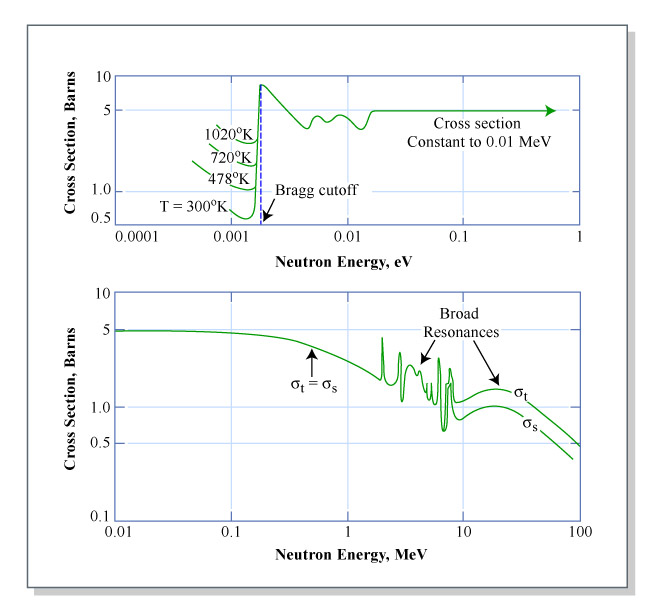
\includegraphics[width=5in]{images/ni/sigma-vs-T.png}
    \caption{Energy Dependence of Total Scattering Cross Section for Graphite\label{sigma-vs-T}}
\end{figure}

\subtopic{Region 1: 1/v}
$E_1 < k_B T$, $v$ is neutron velocity, $V$ is the target nuclear velocity as Maxwellian distribution:
\begin{align}
f(V) &= 4 \pi \left( \frac{M}{2 \pi k_B T} \right)^{3/2} V^2 \exp \left( - \frac{MV^2}{2 k_B T} \right) \\
v \sigma_s (v) &= \int \dV^3 |v-V| \sigma(|v-V|) f(V,T) \\
\sigma_s(v) &= \frac{\sigma_{so}}{\beta^2} \left[ \left(\beta^2 + \frac{1}{2} \right) \mathrm{erf}(\beta) + \frac{1}{\sqrt{\pi}} \beta e^{-\beta^2} \right], \fsp \fsp \beta^2 = \frac{A E}{k_B T}\\
\mathrm{erf}(\beta) &= \int_0^{\beta} \frac{2}{\sqrt{\pi}} e^{-t^2} \dt = 
\begin{dcases*}
\to 0 & $\beta \to 0$ \\
\to 1 & $\beta \to \infty$ 
\end{dcases*} \\
\sigma_s (v) &= 
\begin{dcases*}
\mbox{constant } \frac{\sigma_{so}}{v}& $E \ll k_B T, \beta \ll 1$ \\
\mbox{constant } \sigma_{so}, \mbox{E independent, isotropic} & $E \gg k_B T, \beta \gg 1$ 
\end{dcases*} 
\end{align}
See Figure~\ref{sigma-vs-T-low-energy} for an example of non-crystal water. 
\begin{figure}
    \centering
    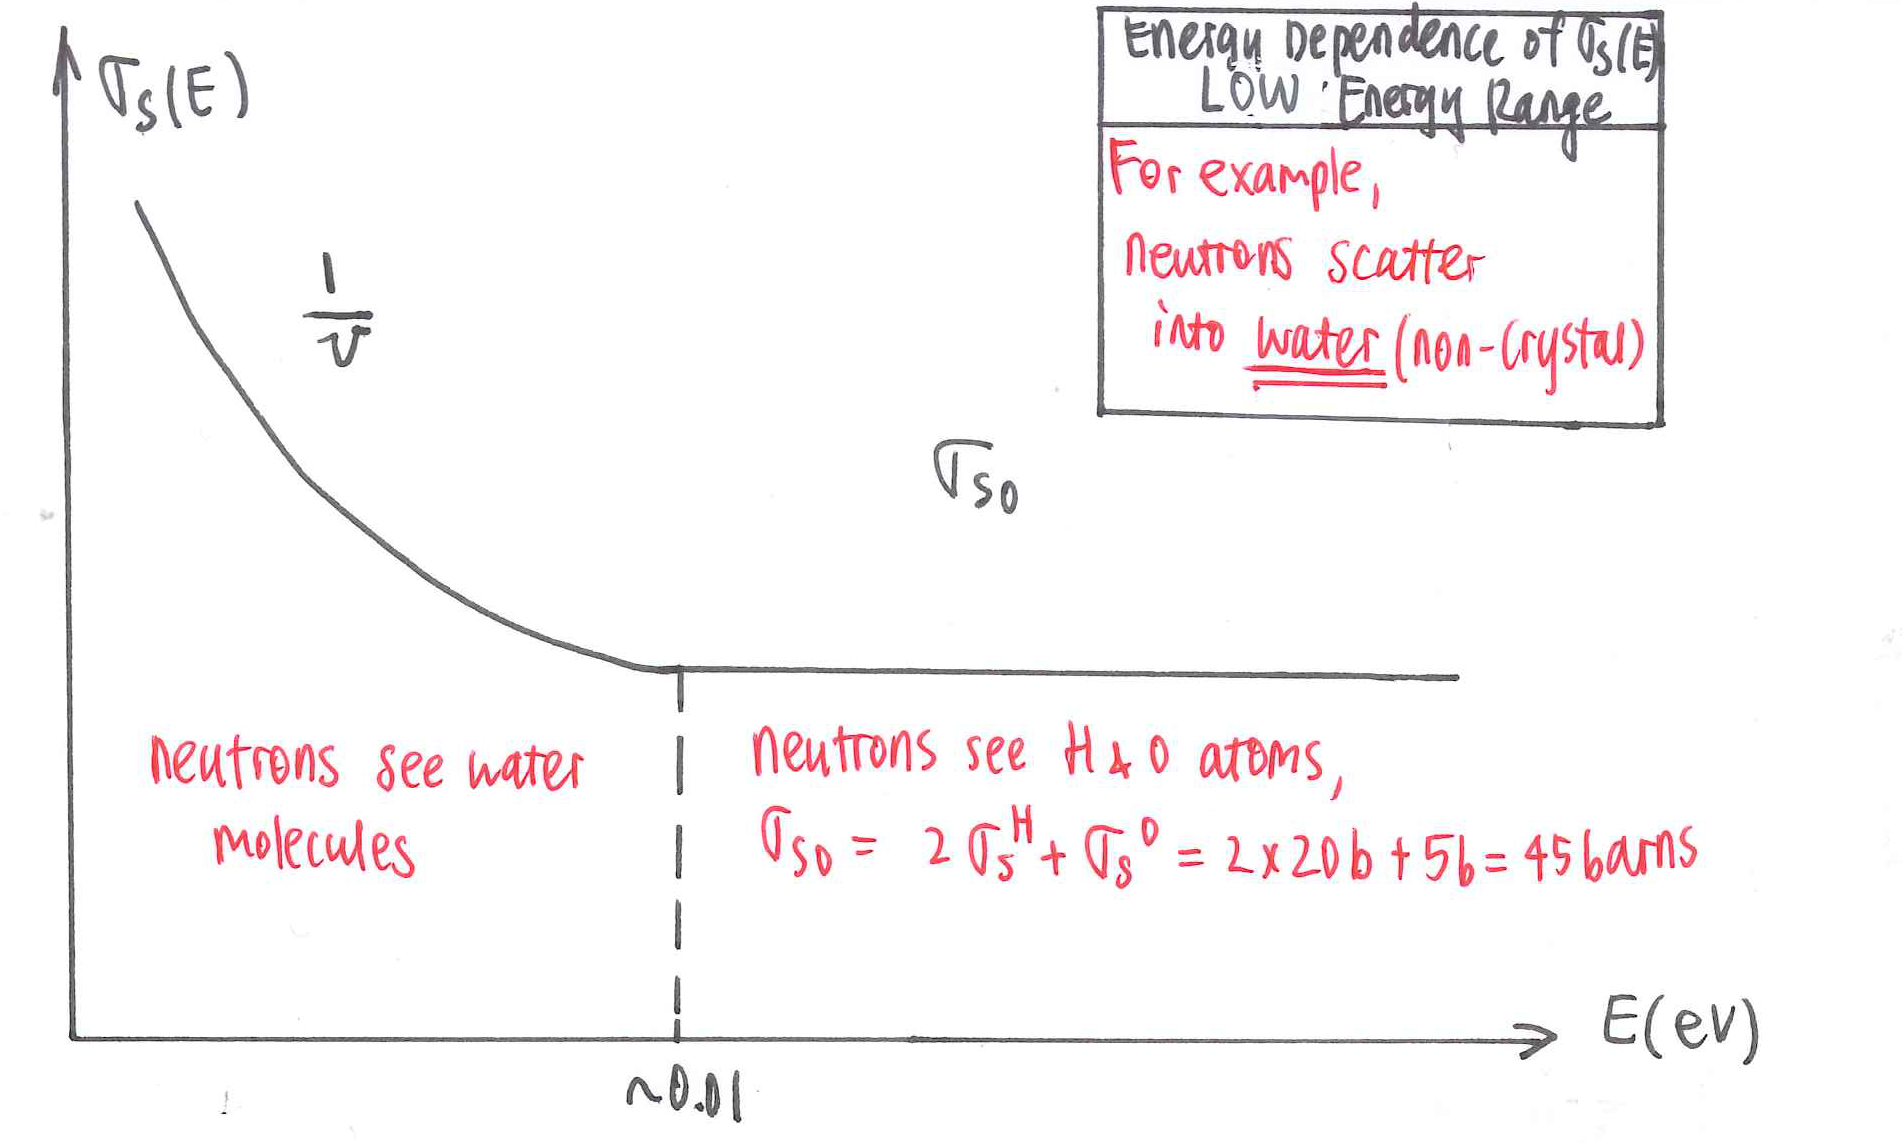
\includegraphics[width=4in]{images/ni/sigma-vs-T-low-energy.png}
    \caption{Scattering Cross Section Depends on Energy, Low Energy Range\label{sigma-vs-T-low-energy}}
\end{figure}

\subtopic{Region 2: Bragg's Law, Only Exist for Crystal Structure} 
Region 2 is low energy like region 1, though region 2 is a result of the inter-planar structure, hence non-crystal material would not have this region, like in Figure~\ref{sigma-vs-T-low-energy}. The wavelength in this region $\lambda_n \approx$ inter-planar spacing; The first spike, in particular, is called \textbf{Bragg-cutoff} whose wavelength is the solution of the Bragg's Law, on the order of $d$ (lattice parameter). 

Each of the later spikes (not as large as the first one though) correspond to smaller lattice spacings, and the reflective waves are constructive interference. Constructive interference (Figure~\ref{constructive-interference}) leads to Bragg's Law, in which $d$ can be along any direction:
\eqn{ 2d \sin \theta = n \lambda} 
\begin{figure}
   \centering
   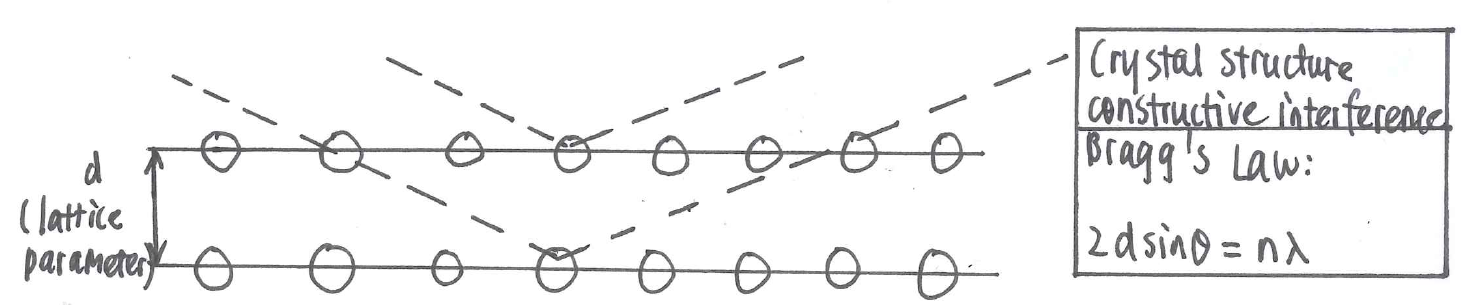
\includegraphics[width=4in]{images/ni/constructive-interference.png}
   \caption{Crystal Structure for Constructive Interference\label{constructive-interference}}
\end{figure}

\subtopic{Region 3: S-wave Scattering} 
Region 3 is the S-wave Potential Scattering range. We have discussed this before 

\subtopic{Region 4: Resonance, Compound Nucleus} 
Region 4 is the Resonance Region; we introduce the `compound nucleus formation' that account for strong interaction between neutron and nucleus that the neutron can penetrate into the nucleus, create disturbance in the nucleus, lead to a intermediate state that include the neutron in the nucleus, and we call this the `Compound Nucleus (CN).' Then the CN would decay. \textcolor{blue}{This formation is used to explain: elastic resonance scattering $(n,n)$; inelastic scattering; radioactive capture $(n,\gamma)$; fission $(n,f)$.} This formation, as shown in Figure~\ref{compound-formation-energy}, typically describes Endothermic Reaction $Q < 0$. It makes sense because the end state has higher energy than the initial state, hence requiring energy input for the process to happen.  
\begin{figure}
   \centering
   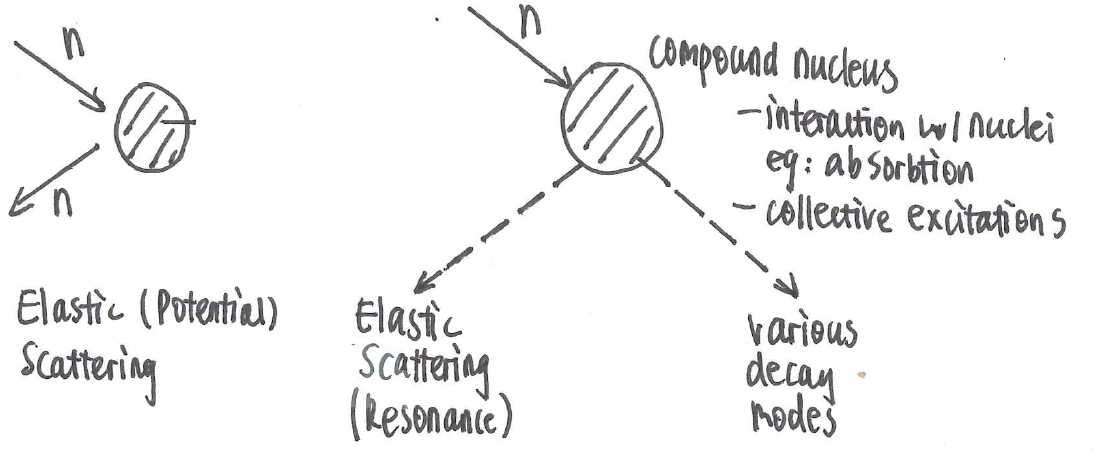
\includegraphics[width=4in]{images/ni/compound-formation.png}
   \caption{Compound Nucleus Formation\label{compound-formation}}
\end{figure}
\begin{figure}
   \centering
   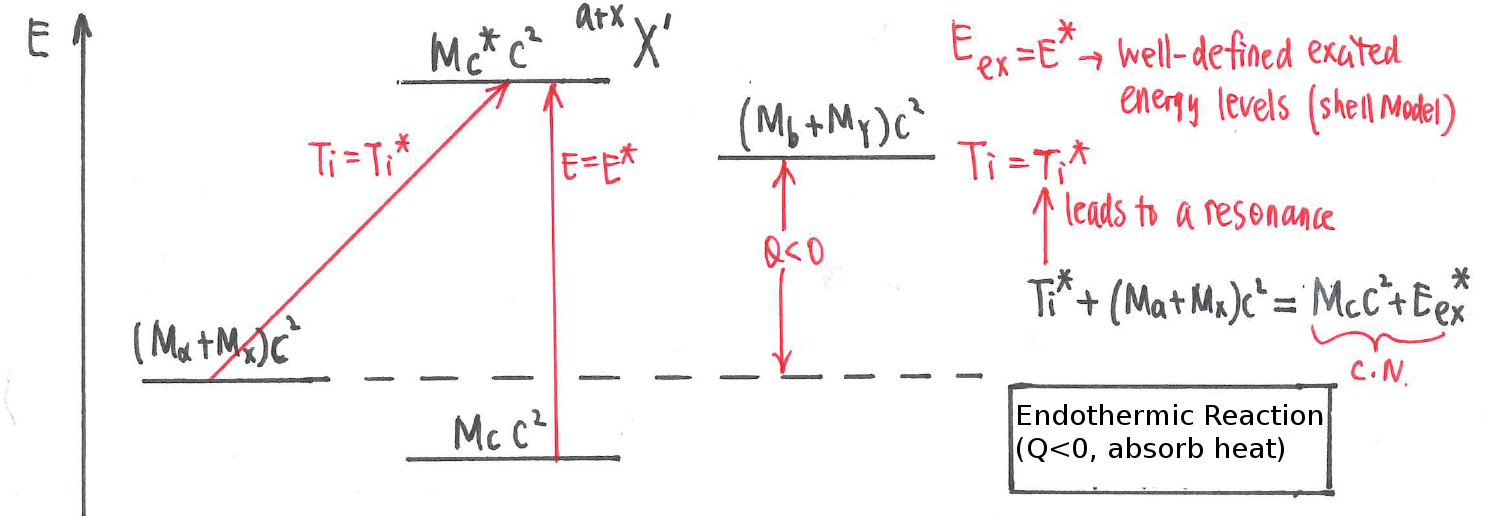
\includegraphics[width=6in]{images/ni/compound-formation-energy.png}
   \caption{Energy Levels in Compound Nucleus Formation\label{compound-formation-energy}}
\end{figure}

$\sigma_C (T_i)$ is the cross-section for CN formation given a KE of $T_i$, $P_b$ is the probability that energy level E would decay by emission of particle. We evaluate the two terms separately (and the two processes: formation and decay decoupled too). 
\begin{align}
a + X  &\to C^* \to b + Y \\
\Aboxed{ \sigma (a,b) &= \sigma_C (T_i) P_b (E) }
\end{align}
where $E$ in $P_b(E)$ is the excitation energy, $P_b(E)$ describes the probability of the decay channel where particle $b$ is emitted characterized by interaction width $\Gamma$, and as explained by Eq.21.12 in SY5, 
\eqn{ \sigma_c (T_i) = \pi \lambda^2 g_J \frac{\Gamma_a \Gamma}{(T_i - T_i^*)^2 + \frac{\Gamma^2}{4}}  }



\begin{enumerate}
\item Elastic Resonance Scattering: \ce{n + ^A_Z X \to \ce{^{A+1}_Z X^*} \to n + ^A_Z X}. See Fig.~\ref{compound-formation-scattering-energy}. 
  \begin{figure}
    \centering
    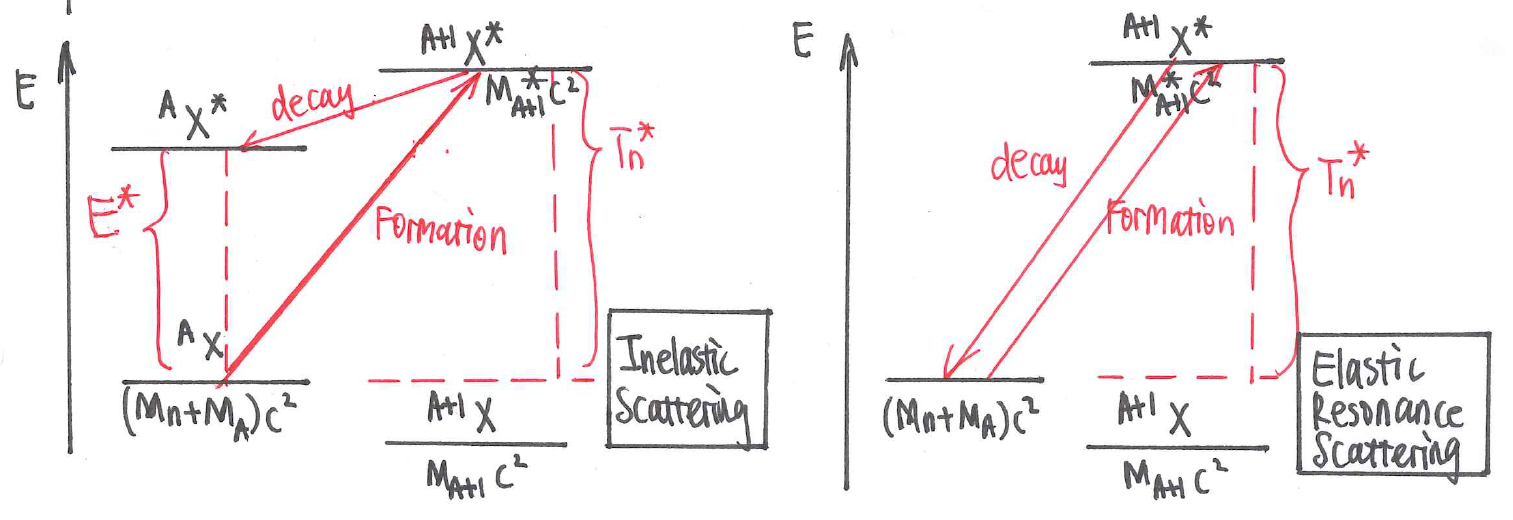
\includegraphics[width=6in]{images/ni/compound-formation-scattering-energy.png}
    \caption{Energy Levels in Resonance Scattering, Elastic and Inelastic\label{compound-formation-scattering-energy}}
  \end{figure}

\item Inelastic Resonance Scattering: \ce{n + ^A_Z X \to \ce{^{A+1}_Z X^*} \to n+ ^A_Z X^*}.

\item Radiative Capture $(n, \gamma)$: 
  \ce{n + ^A_Z X \to \ce{^{A+1}_Z X} \to \gamma + ^{A+1}_Z X}. Notice the neutron is not released.

  Example: \ce{ n+ ^{238} U \to ^{239} U^* \to ^{239} U + \gamma }, in which $E_n = 6.67 \fsp \eV$.
  \begin{figure}
    \centering
    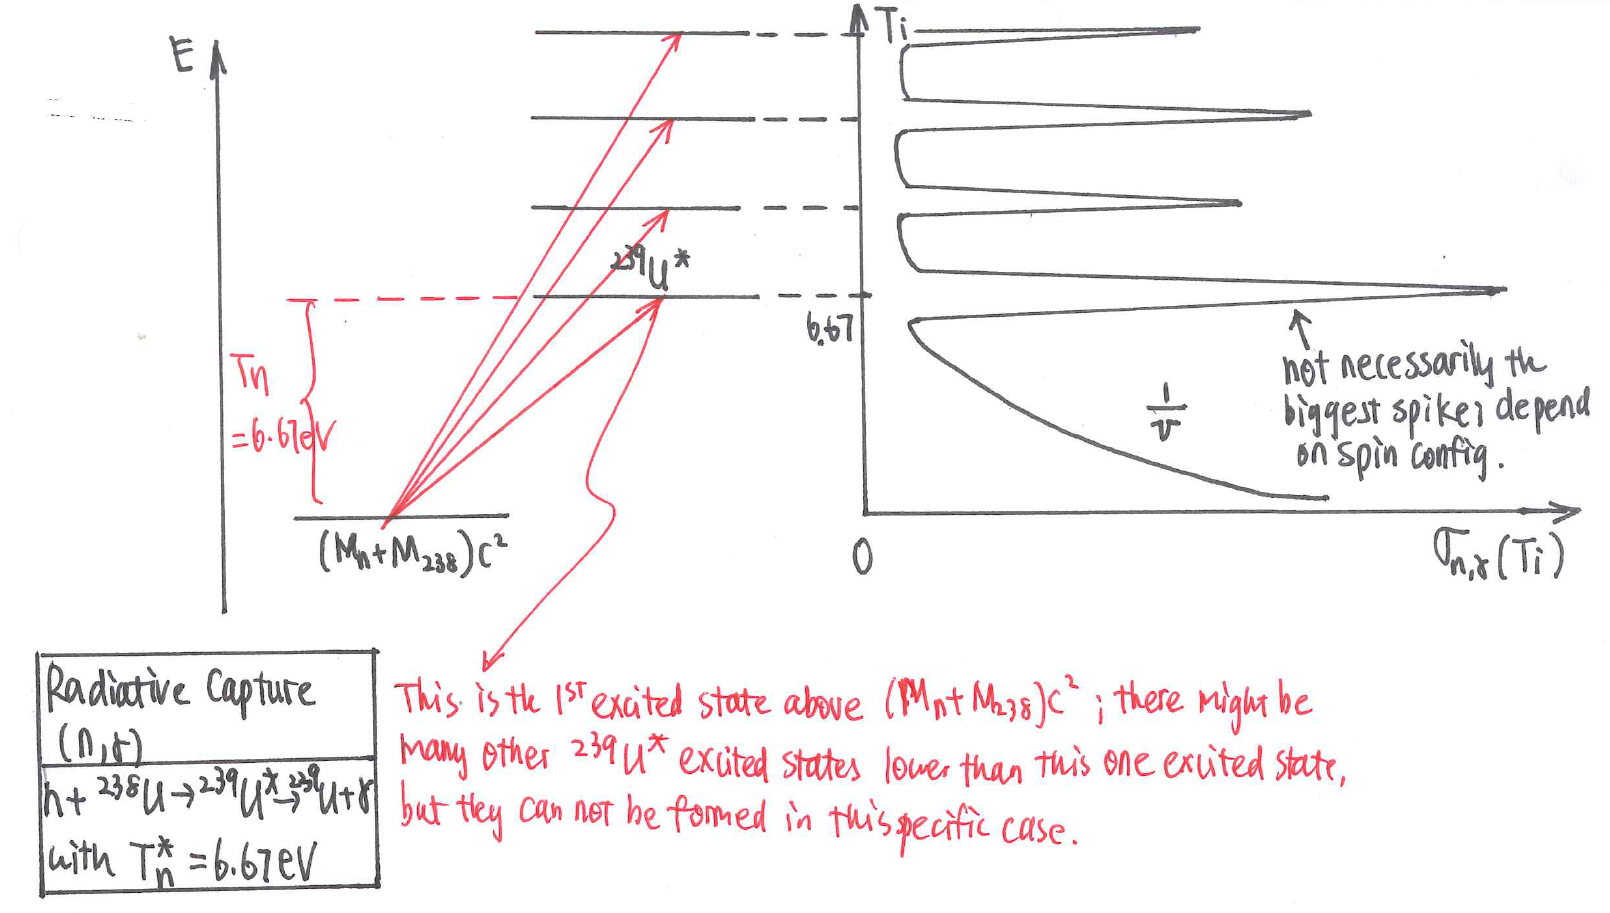
\includegraphics[width=6in]{images/ni/compound-formation-rc-energy.png}
    \caption{Energy Levels in Resonance Scattering, Radiative Capture\label{compound-formation-rc-energy}}
  \end{figure}

  \textbf{Breit-Wigner Single-level Resonance Formula} is used to describe quantitatively the resonance cross-sections, where resonances (or excited state energy levels) are spaced widely apart: 
  \begin{align}
    \sigma_{n, \gamma} (T_i) &= \sigma_0 \frac{\Gamma_n \Gamma_{\gamma}}{(T_i - T_i^*)^2 + \left( \frac{\Gamma}{2} \right)^2} \\
    \Gamma &= \mbox{total line width, the energy width that an excited CN can form about $E^*$;} \\
    \Gamma_{\gamma} &= \mbox{radiative line width, characterizing the probability that the CN will decay with gamma emission;} \\
    \Gamma_n &= \mbox{neutron line width} \propto E^{1/2} \propto v \\
    \sigma_0 &= \mbox{total cross section} = \pi \lambda^2 g \\
    g &= \mbox{statistical spin factor} = \frac{2J + 1}{(2 I_a + 1) (2 I_x + 1)}
  \end{align}
\end{enumerate}


\subtopic{Revisit with SY5}
\begin{enumerate}
\item Absorption cross section can be written as, 
  \eqn{ \sigma (n,\gamma) = \pi \lambda^2 g_J \frac{\Gamma_n \Gamma_{\gamma}}{(T_i - T_i^*)^2 + \frac{\Gamma^2}{4} } }
Absorption behaves like $1/v$ at low wnergy; it has a peak at some $T^*$ with a width. See Fig.~\ref{2167}. 
  \begin{figure}
    \centering
    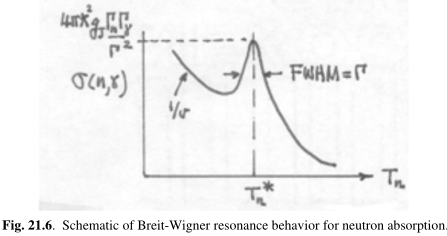
\includegraphics[width=3in]{images/ni/21.6.png}
    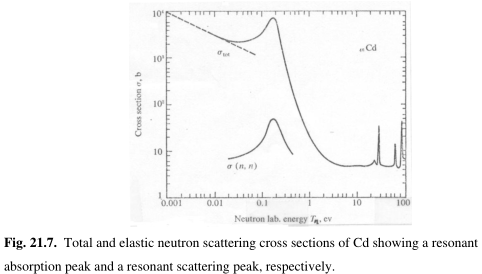
\includegraphics[width=3in]{images/ni/21.7.png}
    \caption{Absorption xs Is 1/v Before Resonances}  \label{2167}
  \end{figure}

\item Elastic scattering\footnote{SY5 Eq.21.15, Fig.21.8/9}:
\eqn{ \gamma(n,n) = 4 \pi a^2 + \pi \lambda^2 g_J \frac{\Gamma_n^2}{(T_i - T_i^*)^2 + \frac{\Gamma^2}{4} } + 4 \pi \lambda g_J a \Gamma_n \frac{T_i - T_i^*}{(T_i - T_i^*)^2 + \frac{\Gamma^2}{4} } }
 There are three terms: potential ($4\pi a^2$), resonance, and the interference between the two. The interference is responsible for the destructive behavior (decreasing in value) right before a resonance, which differs from absorption's resonances which is just $1/v$ instead of a destructive behavior. See Fig.~\ref{2189}. 
    \begin{figure}
    \centering
    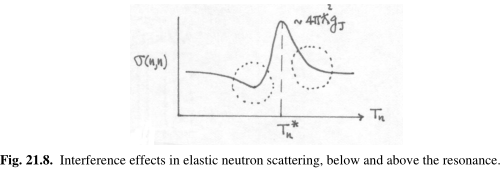
\includegraphics[width=4in]{images/ni/21.8.png}
    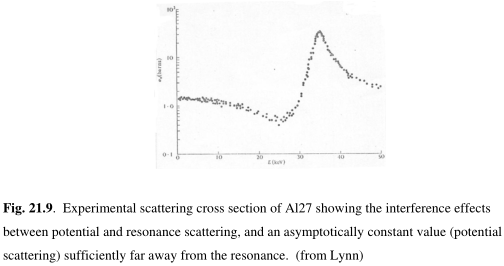
\includegraphics[width=4in]{images/ni/21.9.png}
    \caption{Scattering xs Is Destructive Before Resonances}  \label{2189}
  \end{figure}

\item Fission: see SY10. 
\end{enumerate}


\end{document}
